\section{\huge{Bonusopgaver}}

\subsection{Den hyggelige opgave}

Forbind prikkerne.

\begin{center}
\includegraphics[width=.99\textwidth]{forbind-prikkerne.pdf}
\end{center}


\newpage

\subsection{Den XXX opgave}


\newpage

\subsection{Den YYY opgave}


\newpage

\subsection{Den komprimerende opgave}

Her er et eksempel på en bankoplade:

\begin{center}
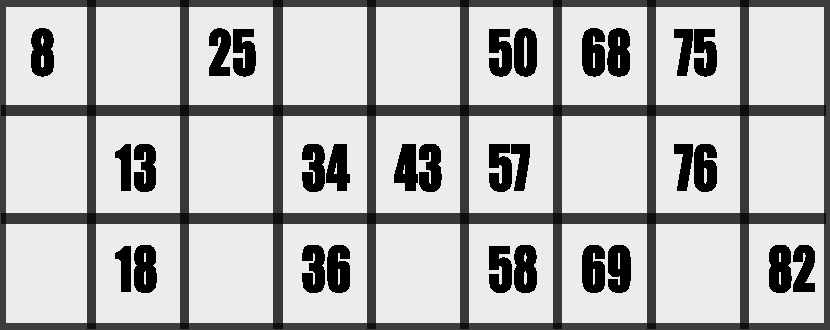
\includegraphics[width=.99\textwidth]{bankoplade.pdf}
\end{center}

Der er vigtige regler for bankoplader.  Her er de\footnote{Nils Andersen.  Hvor
mange bankoplader er der?  2003.\\
\tiny{\url{http://sprutskalle.dk/blog/wp-content/uploads/bankoplader.pdf}}}:

\begin{itemize}
\item Der benyttes numrene fra og med 1 til og med 90.
\item En bankoplade har 3 rækker og 9 søjler.
\item En plade har 15 forskellige numre og 12 tomme felter.
\item Der er mindst et nummer i hver søjle og præcis fem numre i hver række.
\item Den første søjle (fra venstre), kaldt $s_0$, kan have numrene fra og med
$1$ til og med $9$.  Den sidste søjle, kaldt $s_8$, kan have numrene fra og med
$80$ til og med $90$.  Hver søjle $s_n$, hvor $1 \leq n \leq 7$, kan have
numrene fra og med $10n$ til og med $10n + 9$.
\end{itemize}

\textbf{Underopgave 0:} Tjek at den givne eksempelplade opfylder de fem krav.

\textbf{Underopgave 1:} Opfind en algoritme til at komprimere en bankoplade
effektivt, dvs. at repræsentere en bankoplade på få bits (uden tab af
information!).


\newpage

\subsection{Den skægge opgave}

% The Collatz conjecture

Her er en funktion for et vilkårligt tal $n$:
\begin{align*}
f(n) = \begin{cases}
n/2 &\text{hvis }n\text{ er lige}\\
3n + 1 &\text{hvis }n\text{ er ulige}\\
\end{cases}
\end{align*}
For eksempel er $f(10) = 5$ og $f(7) = 22$.

Her er en talfølge -- baseret på funktionen $f$ -- der begynder med et
vilkårligt tal $n$:
\begin{align*}
a_i = \begin{cases}
n &\text{når }i = 0\\
f(a_{i - 1}) &\text{når }i > 0\\
\end{cases}
\end{align*}
Hvis vi for eksempel sætter $n = 12$, får vi talfølgen
$a_0 = 12, a_1 = 6, a_2 = 3, a_3 = 10, a_4 = 5, a_5 = 16, a_6 = 8, a_7 = 4, a_8
= 2, a_9 = 1$.  Vi stopper med at vise en talfølge når den når tallet $1$, for
$1$ er et pænt tal, og $f(f(f(1))) = 1$ (vis dette), så den vil alligevel blot
gentage sig.

\textbf{Din opgave:} Bevis eller modbevis følgende formodning:
\begin{quote}
Ligemeget hvilket starttal $n$ der vælges, vil talfølgen altid nå tallet $1$.
\end{quote}

\textbf{\emph{NB: Der udloddes en flaske snaps til den første som kommer op i
baren med en korrekt besvarelse af denne opgave!}}
